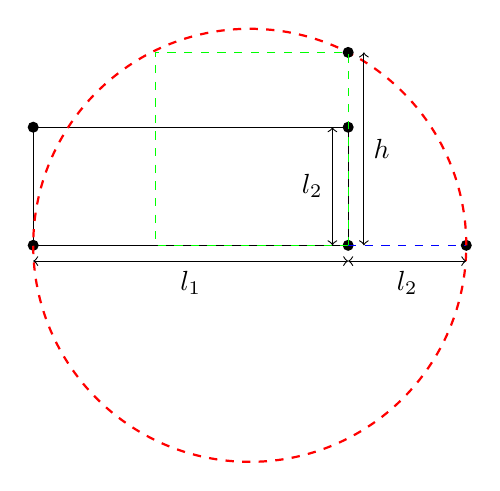
\begin{tikzpicture}

\coordinate (A) at (-2, 0);
% \node at (A) [below]{$A$};
\fill (A)  circle[radius=2pt];

\coordinate (B) at (2,0);
% \node at (B) [below]{$B$};
\fill (B)  circle[radius=2pt];

\coordinate (C) at (2,1.5);
% \node at (C) [above]{$C$};
\fill (C)  circle[radius=2pt];

\coordinate (D) at (-2,1.5);
% \node at (D) [above]{$D$};
\fill (D)  circle[radius=2pt];

\coordinate (C2) at (3.5,0);
% \node at (C2) [right]{$C2$};
\fill (C2)  circle[radius=2pt];

\draw (A) -- (B) -- (C) -- (D) -- (A); 
\tkzDrawArc[R, color=blue,dashed,thick](B, 1.5cm)(0,90);
\draw [dashed, color=blue] (B) -- (C2);

\draw[red,thick,dashed] (0.75,0) circle (2.75);

\coordinate (H) at (2,2.45);
% \node at (H) [right]{$H$};
\fill (H)  circle[radius=2pt];

\draw [<->] (2.2,0) -- (2.2,2.45)  node[midway, right]{$h$};
\draw [<->] (-2,-0.2) -- (2,-0.2)  node[midway, below]{$l_1$};
\draw [<->] (1.8,0) -- (1.8,1.5)  node[midway, left]{$l_2$};
\draw [<->] (2,-0.2) -- (3.5,-0.2)  node[midway, below]{$l_2$};
\draw [color = green, dashed] (B) -- (H) -- (-0.45,2.45) -- (-0.45,0) -- (B);
% \draw [dashed] (A) -- (H);

\end{tikzpicture}